\documentclass[useAMS,usenatbib]{mnras}
\pdfminorversion=4

% The following is needed to fix the margins if using Letter-size paper
% REMOVE if your LaTeX uses A4 paper by default
\addtolength\topmargin{-1.8cm}
\usepackage{newtxtext}
\usepackage[varg]{newtxmath}

\usepackage{graphicx}
\usepackage{booktabs}
\usepackage{siunitx}
\bibliographystyle{mnras}
%\usepackage{astrojournals}
\usepackage{fixltx2e}


% \newcounter{ion}
% \newcommand\fakesc[1]{\protect\scalebox{1.0}[0.8]{#1}}
% \newcommand\ION[2]{\ensuremath{\mathrm{#1\,\fakesc{#2}}}}
% \newcommand\ion[2]{\setcounter{ion}{#2}\ION{#1}{\Roman{ion}}}
\newcommand\hii{\ion{H}{ii}}
\newcommand\oi{[\ion{O}{i}]}
\newcommand\oiii{[\ion{O}{iii}]}
\newcommand\nii{[\ion{N}{ii}]}
\newcommand\sii{[\ion{S}{ii}]}
\newcommand\siii{[\ion{S}{iii}]}
\newcommand\ha{\ensuremath{\mathrm{H\alpha}}}
\newcommand\kms{\ensuremath{\mathrm{km\ s^{-1}}}}
\newcommand\los{\ensuremath{_{\mathrm{los}}}}
\newcommand\pos{\ensuremath{_{\mathrm{pos}}}}
\newcommand\obs{\ensuremath{_{\mathrm{obs}}}}
\newcommand\ins{\ensuremath{_{\mathrm{ins}}}}
\newcommand\rms{\ensuremath{_{\mathrm{rms}}}}
\newcommand\turb{\ensuremath{_{\mathrm{turb}}}}
\newcommand\FS{\ensuremath{_{\mathrm{fs}}}}
\newcommand\therm{\ensuremath{_{\mathrm{therm}}}}

\newcommand\Efrac{\ensuremath{_{\scriptscriptstyle E/E_0}}}
\newcommand\denfrac{\ensuremath{_{\scriptscriptstyle \rho/\rho_0}}}
\newcommand\lnSfrac{\ensuremath{_{\scriptscriptstyle \ln S/S_0}}}
\newcommand\Sfrac{\ensuremath{_{\scriptscriptstyle S/S_0}}}

\title{Will's new version of abstract}


\begin{document}
\maketitle

\begin{abstract}
  In order to study the nature, origin, and impact of turbulent
  velocity fluctuations in the ionized gas of the Orion Nebula, we
  apply a variety of statistical techniques to observed velocity
  cubes.  The cubes are derived from high resolving power
  (\(R \approx 40\,000\)) longslit spectroscopy of optical emission
  lines spanning a range of ionizations and covering the central
  $3^\prime \times 5^\prime$ of the nebula. From Velocity Channel
  Analysis (VCA), we find that the slope of the velocity power
  spectrum is consistent with predictions of Kolmogorov theory between
  scales of 8 and 22 arcsec (0.02 to 0.05~pc).  The outer scale, which
  is the dominant scale of density fluctuations in the nebula,
  approximately coincides with the autocorrelation length of the
  velocity fluctuations that we determine from the second order
  velocity structure function.  We propose that this is the principal
  driving scale of the turbulence, which originates in the
  autocorrelation length of dense cores in the Orion molecular
  filament.  By combining analysis of the non-thermal line widths with
  the systematic trends of velocity centroid versus ionization, we
  find that the global champagne flow and smaller scale turbulence
  each contribute in equal measure to the total velocity dispersion,
  with respective RMS widths of \(4\)--\(5~\kms\).  The turbulence is
  subsonic and can account for only one half of the derived variance
  in ionized density, with the remaining variance provided by density
  gradients in photoevaporation flows from globules and filaments.
\end{abstract}

\addtocounter{section}{4}
\addtocounter{subsection}{2}
\subsection{What is the significance of the 22 arcsec and 8 arcsec
  length scales?}
\label{sec:what-significance-22}

The velocity channel analysis suggests that two length scales are
important in the Orion Nebula, corresponding to the limits of
regime~II (see Fig.~5). The break in power law at 22~arcsec and
8~arcsec occurs for both thin and thick velocity slices. This
indicates that it is a feature of the emissivity power spectrum, and
not the velocity power spectrum. Below 8~arcsec (regime~III), the
emissivity power spectrum is very steep in all the lines, indicating
that small-scale fluctuations are relatively unimportant.  Above
22~arcsec (regime~I), the power spectrum \(P(k)\) is very flat,
similar to the noise-dominated spectrum in regime~IV, suggesting that
fluctuations are relatively uncorrelated on larger scales.  This is
underlined by the analysis in Appendix~\ref{sec:toy-model-surface},
where it is shown that a combination of Gaussian brightness peaks with
widths (FWHM) from \(\approx 4''\) and \(12''\) can capture the broad
features of the observed power spectra.% \footnote{The factor of two
  % difference between these widths and the length scales discussed
  % earlier in the paragraph is because a fluctuation consists of both
  % a peak and a trough, and so the width of the peak is only one half
  % of the fluctuation wavelength.}

The outer scale of \(22''\) coincides with scale where the structure
functions reach a value of unity (Fig.~8), which corresponds to the
correlation length, \(l_0\), of the velocity fluctuations (see
Fig.~14).  It is therefore plausible to associate this scale, which
corresponds to a physical size of \(\approx 0.05\)~parsec, with the
driving scale of turbulence in the nebula.  The inner scale of
\(8''\), corresponding to a physical size of \(\approx 0.02\)~parsec,
is harder to associate with any particular process since the structure
functions (Fig.~8) show no apparent feature at this scale.

\subsection{Does velocity turbulence cause the surface brightness
  fluctuations?}
\label{sec:does-veloc-turb}

The surface brightness fluctuations on the plane of the sky are
primarily caused by emissivity fluctuations within the nebular volume,
which are in turn caused by fluctuations in electron density,
temperature, and ionization.  The temperature and ionization
dependence of the emissivity is very different for each line, but the
electron density dependence is similar in all cases, being
\(\propto N_e^2\) in the low density limit, which is appropriate for
all but the \sii{} lines.  It therefore seems likely that any
\emph{commonalities} in the power spectra between all the different
emission lines will give us information about the electron density
fluctuations within the nebula.

In \S~\ref{sec:turb-contr-spectr} it was shown that the rms fractional
surface brightness variation in 2D is \(\sigma\Sfrac \approx 0.5\) for
all lines, and the rms emissivity variation in 3D is predicted to be
\(\sigma\Efrac = \xi \sigma\Sfrac\), where the ``de-projection
factor'' is \(\xi = 2\)--\(3\) \citep{Brunt:2010a}.  On the other
hand, if the emissivity fluctuations are due to variations in the
density squared, then the rms fractional 3D density variation is
\(\sigma\denfrac = 0.5\, \sigma\Efrac\), which approximately cancels
out the de-projection factor so that
\(\sigma\denfrac \approx \sigma\Sfrac \approx 0.5\).  If the density
fluctuations are \emph{caused} by the turbulent velocity fluctuations,
then numerical simulations \citep{Konstandin:2012a} show that there is
a linear relationship between \(\sigma\denfrac\) and the rms Mach
number, \(M\), of the turbulence: \(\sigma\denfrac = b M\), where
\(b = 1/3\) to \(b = 1\), depending on whether the turbulent driving
is primarily solenoidal or compressive.  The rms Mach number is the
ratio of the velocity dispersion to the ionized isothermal sound speed
\(M = \sigma_u / c_i\), where \(\sigma_u = \sigma\turb \approx 4~\kms\)
(see \S~3.4) and \(c_i \approx 11~\kms\).  Thus, \(M \approx 0.35\)
so that, given \(b < 1\), an upper limit to the turbulent contribution to the
density fluctuations is \(\sigma\denfrac \la 0.35\). 

Furthermore, the slopes of the surface brightness fluctuation spectra
in regime~II are significantly shallower than expected from a top-down
turbulent cascade in the subsonic limit \citep{Konstandin:2015a}.  A
similar result is seen in our numerical simulations (see \S~4.2), with
the important difference that in the simulation the velocity spectrum
is also shallow, whereas the thin-slice VCA analysis for the
observations (\S~3.3.1) is consistent with a Kolmogorov slope for the
velocity fluctuation spectrum in regime~II.

We therefore require a further mechanism to explain the roughly 50\%
of the variance in ionized density that cannot be accounted for by
turbulent velocity fluctuations.  This could plausibly be provided by
the bright-rimmed structure of the photoevaporation flows away from
dense molecular globules and filaments (e.g., \citep{Bertoldi:1990a,
  Henney:2009b}), which are responsible for driving the turbulence.
We have calculated the emissivity-weighted density PDF for a simple
model of a single spherically divergent, isothermal evaporation flow
from a D-critical ionization front \citep{Dyson:1968a} and find
\(\sigma\denfrac = 0.56\).  For an an ensemble of such flows with
varying peak densities the \(\sigma\denfrac\) would be even higher, so
that in order for their global contribution to rival that of the
velocity fluctuations it is sufficient that a fraction
\(0.1\)--\(0.5\) of the total emission should come from such flows.


% problems with this
% scenario are apparent once the power spectrum towards smaller scales
% (higher wavenumbers) is considered.  The thin-slice VCA analysis
% (\S~3.3.1) is consistent with a Kolmogorov slope for the velocity
% fluctuation spectrum in regime~II, with power law index
% \(n \approx -3.67\).  For subsonic turbulence, analytic
% \citep{Saichev:1996a} and numerical studies \citep{Konstandin:2015a}
% show that the density power spectrum should be even steeper,
% \(n \approx -4\).

% Since all the relationships in the chain
% \(\sigma_u \to M \to \sigma\denfrac \to \sigma\Efrac \to
% \sigma\Sfrac\) are linear, it follows that the surface brightness
% fluctuations should also have the same slope, so long as all the
% coefficients in those linear relationships are independent of scale.
% The observed slopes are in fact considerably shallower than the
% Kolmogorov value, with indices \(n = -2.6\) to \(-3\), depending on
% the emission line.  A turbulent explanation for the slope therefore
% requires that either \(b\) should increase with wavenumber, \(k\), or
% that \(\xi\) should decrease with \(k\).  The first is impossible
% because \(b\) is already assumed to have its maximum value.  The
% second is more plausible, since 

\appendix

\addtocounter{section}{4}
\section{Toy model of surface brightness profiles}
\label{sec:toy-model-surface}
\begin{figure}
  \centering
  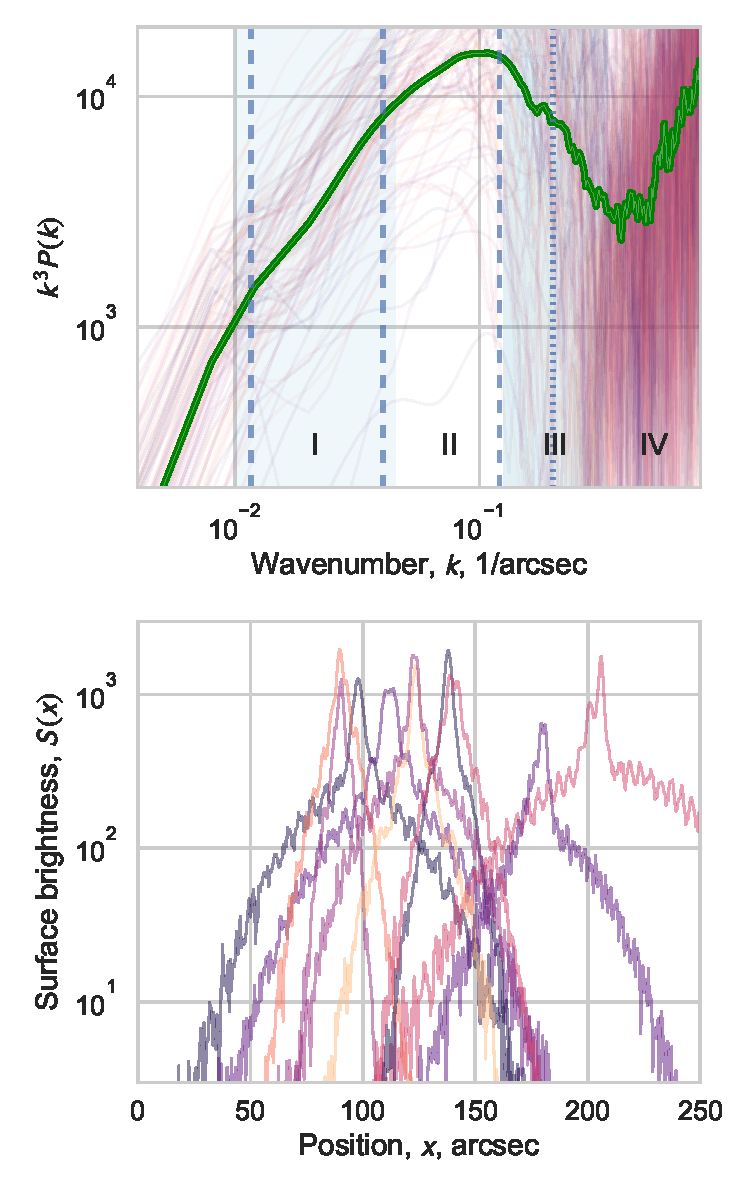
\includegraphics[width=\linewidth]{fake-powerspec}
  \caption{Compensated power spectra (upper panel) of 100 fake
    one-dimensional surface brightness profiles.  Individual power
    spectra are shown as faint lines, while the the thick green line
    shows the average spectrum.  The lower panel shows an example of
    10 of the brightness profiles on a semi-logarithmic scale.}
  \label{fig:fake-powerspec}
\end{figure}

To try and gain insight into the observed power spectra, we have
determined the simplest emission model that can reproduce the
qualitative features of regimes I--IV.  The emission model is
illustrated in Figure~\ref{fig:fake-powerspec} and consists of the
following spatial components:
\begin{enumerate}
\item A narrow Gaussian with peak brightness 800 (\(\pm 30\%\)) and FWHM
  \(4''\) (\(\pm 30\%\)).
\item A broader Gaussian with peak brightness 400 (\(\pm 30\%\)) and
  FWHM \(12''\) (\(\pm 30\%\)).
\item A very broad Gaussian with peak brightness 240 (\(\pm 30\%\)) and
  FWHM \(88''\) (\(\pm 50\%\)). 
\item A sinusoidal variation with wavelength \(5''\) (\(\pm
  50\%\)) and relative amplitude 15\%, which multiplies the sum of
  components (i)--(iii). 
\item Poisson \(\sqrt{N}\) noise, assuming that the brightness is in
  units of counts/pixel.
\end{enumerate}
The wavenumber \(k =
1/\lambda\) of each component is
indicated by vertical lines on the power spectrum shown in the upper
panel of Figure~\ref{fig:fake-powerspec} (dashed lines for the
Gaussian components (i)--(iii), dotted lines for the sinusoidal
component (iv)). For the Gaussian components, we assume \(\lambda
\approx 2 \times \mathrm{FWHM}\) since the Gaussian peak represents
only half of a fluctuation wavelength. 

Components (i) and (ii) are chosen so as to reproduce regime~II in the
power spectra of \S~3.1, with a relatively shallow slope
(\(\gamma > -3\)) between scales of 8\(''\) and 22\(''\).  As is, the
model best represents the \nii{} power spectrum (upper right panel of
Fig.~5), but the precise value of the slope can be controlled by
varying the relative strength of the narrow (\(4''\)) and the broader
(\(12''\)) component.  For example, the \oiii{} power spectrum
requires nearly equal amplitudes for these two components.  

With only components (i) and (ii), the model power spectrum is too shallow
in regime~I (with \(\gamma \approx 0\)) and is too steep in
regime~III, showing a deep minimum in the \(k^3 P(k)\) curve before
arriving at the noise-dominated regime~IV.  These minor deficiencies are
ameliorated by the introduction of the secondary components~(iii)
and~(iv), respectively. 

The average power spectrum from 100 realizations of the toy model is
calculated, where the brightness and width of each component is chosen
according to normal distributions with central value (\(\pm\) RMS \%
variation) as given above.  The result is in remarkably good agreement
with the observed power spectra, except that the observations tend to
show sharper breaks at the boundaries between the different
regimes. It should be emphasized that the toy model is only an
idealization of the spatial variations present in the real surface
brightness maps, which typically show \(\sim 10\) prominent peaks in
each one-dimensional slit profile, rather than the single peak of the
model.



\bibliography{BibdeskLibrary-slavoj}

\end{document}
%%% Local Variables:
%%% mode: latex
%%% TeX-master: t
%%% End:
